\subsection{}
The short run function can take any number of shapes.\\
No workers, no matter the capital, bring no output.\\
As you hire more and more workers, at first the output increases at an increasing rate, then slows down.
\begin{figure}[H]
    \centering
    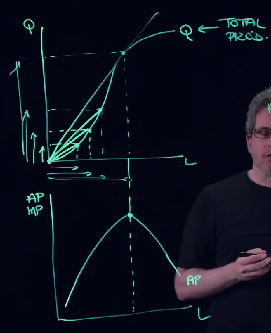
\includegraphics[width=0.5\textwidth]{Chapter7/ShortRun.png}
    \caption{Short Run Production Function}
\end{figure}
\begin{equation}
    \text{Average Production (AP)}= \frac{TP}{L} = \frac{Q}{L}
\end{equation}
The slope of the line from the origin to any point on the short run production curve is the average production.\\
Marginal production is the benefit from hiring one more worker.
\begin{equation}
    \text{Marginal Production (MP)} = \frac{\Delta TP}{\Delta L} = \frac{\Delta Q}{\Delta L}
\end{equation}
One worker means everything they produce is marginal production and the average production.\\
Therefore average production and marginal production are equal at the beginning of the curve.\\
If the average rises, the marginal is above the average.\\
At the maximum point of the average production, the marginal production is equal to the average production.
\begin{figure}[H]
    \centering
    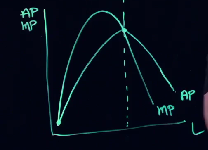
\includegraphics[width=0.5\textwidth]{Chapter7/AverageAndMarginalProduction.png}
    \caption{Short Run Average and Marginal Production}
\end{figure}
We can also see the short run in a table.
\begin{figure}[H]
    \centering
    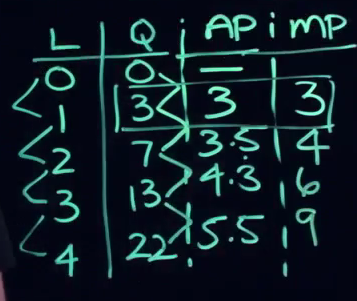
\includegraphics[width=0.5\textwidth]{Chapter7/ShortRunTable.png}
    \caption{Short Run Production Table}
\end{figure}